\documentclass[tikz,border=10pt]{standalone}
\usepackage{sansmath}
\usepackage{siunitx}

\begin{document}
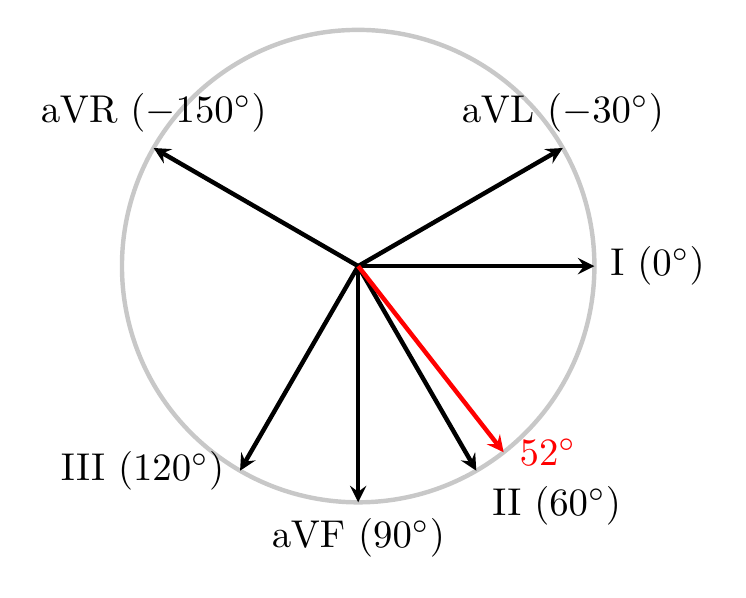
\begin{tikzpicture}

\def\size{3}
\def\textsize{1.4}
\definecolor{brightgray}{RGB}{200,200,200}
\coordinate (center) at (0, 0);

\draw[ultra thick, brightgray] (center) circle (\size cm);

\draw[ultra thick, ->, >=stealth] (center) --  ({\size*cos(0)}, {-\size*sin(0)}) node[right, scale=\textsize] {I ($\ang{0}$)};

\draw[ultra thick, ->, >=stealth] (center) -- ({\size*cos(60)}, {-\size*sin(60)}) node[below right, scale=\textsize] {II ($\ang{60}$)};

\draw[ultra thick, ->, >=stealth] (center) -- ({\size*cos(120)}, {-\size*sin(120)}) node[left, scale=\textsize] {III ($\ang{120}$)};

\draw[ultra thick, ->, >=stealth] (center) -- ({\size*cos(90)}, {-\size*sin(90)}) node[below, scale=\textsize] {aVF ($\ang{90}$)};

\draw[ultra thick, ->, >=stealth] (center) -- ({\size*cos(-30)}, {-\size*sin(-30)}) node[above, scale=\textsize] {aVL ($\ang{-30}$)};

\draw[ultra thick, ->, >=stealth] (center) -- ({\size*cos(-150)}, {-\size*sin(-150)}) node[above, scale=\textsize] {aVR ($\ang{-150}$)};

\draw[ultra thick, ->, >=stealth, red] (center) -- ({\size*cos(52)}, {-\size*sin(52)}) node[right, scale=\textsize] {$\ang{52}$};

\end{tikzpicture}
\end{document}